\documentclass[11pt]{article}

% ------------------------------------------------------------
% Standard LaTeX packages
% ------------------------------------------------------------
\usepackage[margin=1in]{geometry}
\usepackage{amsmath,amssymb,mathtools}
\usepackage{amsthm}
\usepackage[american]{babel}
\usepackage{stmaryrd}
\usepackage{enumitem}
\usepackage{booktabs}
\usepackage{array}
\usepackage{listings}
\usepackage[x11names,table]{xcolor}
\usepackage{mdframed}
\usepackage{tikz}
\usetikzlibrary{arrows.meta,positioning,calc,decorations.pathmorphing}
\usepackage{url}
\usepackage[colorlinks=true,linkcolor=blue,citecolor=blue,urlcolor=blue]{hyperref}

% ---------- Theorem environments ----------
\theoremstyle{plain}
\newtheorem{theorem}{Theorem}[section]
\newtheorem{proposition}[theorem]{Proposition}
\newtheorem{lemma}[theorem]{Lemma}
\newtheorem{corollary}[theorem]{Corollary}
\newtheorem{conjecture}[theorem]{Conjecture}

\theoremstyle{definition}
\newtheorem{definition}[theorem]{Definition}
\newtheorem{axiombox}[theorem]{Axiom}
\newtheorem{protocol}[theorem]{Protocol}
\newtheorem{example}[theorem]{Example}

\theoremstyle{remark}
\newtheorem{remark}[theorem]{Remark}

% ---------- Notation ----------
\newcommand{\N}{\mathbb{N}}
\newcommand{\Z}{\mathbb{Z}}
\newcommand{\Q}{\mathbb{Q}}
\newcommand{\R}{\mathbb{R}}
\newcommand{\C}{\mathbb{C}}
\newcommand{\F}{\mathbb{F}}
\newcommand{\calO}{\mathcal{O}}
\newcommand{\calL}{\mathcal{L}}
\newcommand{\Gal}{\mathrm{Gal}}
\newcommand{\GL}{\mathrm{GL}}
\newcommand{\SL}{\mathrm{SL}}
\newcommand{\Sp}{\mathrm{Sp}}
\newcommand{\GSp}{\mathrm{GSp}}
\newcommand{\End}{\mathrm{End}}
\newcommand{\Frob}{\mathrm{Frob}}
\newcommand{\CRM}{\mathrm{CRM}}
\newcommand{\tr}{\mathrm{tr}}
\newcommand{\rk}{\mathrm{rk}}
\newcommand{\Gr}{\mathrm{Gr}}
\newcommand{\Sym}{\mathrm{Sym}}
\newcommand{\Ggal}{G_{\mathrm{gal}}}
\newcommand{\NS}{\mathrm{NS}}
\newcommand{\Pic}{\mathrm{Pic}}
\newcommand{\Gm}{\mathbb{G}_{\mathrm{m}}}
\newcommand{\MT}{\mathrm{MT}}

\newcommand{\BISH}{\ensuremath{\mathsf{BISH}}}
\newcommand{\LPO}{\ensuremath{\mathsf{LPO}}}
\newcommand{\WLPO}{\ensuremath{\mathsf{WLPO}}}
\newcommand{\LLPO}{\ensuremath{\mathsf{LLPO}}}
\newcommand{\MP}{\ensuremath{\mathsf{MP}}}
\newcommand{\FT}{\ensuremath{\mathsf{FT}}}
\newcommand{\CLASS}{\ensuremath{\mathsf{CLASS}}}
\newcommand{\CBN}{\mathrm{CBN}}
\newcommand{\HdR}{H^1_{\mathrm{dR}}}
\newcommand{\PF}{\mathrm{PF}}

% ---------- Code listing style for Lean ----------
\definecolor{codegreen}{rgb}{0,0.6,0}
\definecolor{codegray}{rgb}{0.5,0.5,0.5}
\definecolor{codepurple}{rgb}{0.58,0,0.82}
\definecolor{backcolour}{rgb}{0.95,0.95,0.92}

\lstdefinelanguage{Lean}{
  keywords={theorem, lemma, def, definition, axiom, structure, class, instance,
            by, exact, intro, intros, apply, refine, constructor, use, obtain,
            have, show, from, fun, assume, let, in, if, then, else,
            match, with, end, namespace, section, variable, variables,
            example, begin, sorry, admit, noncomputable, classical,
            import, open, export, private, protected, mutual, meta,
            do, for, while, return, try, catch, finally,
            Type, Prop, Sort, Type*, forall, exists, where, extends,
            set, push_neg, rw, simp, omega, nlinarith, linarith, ring,
            ext, rfl, congr, fin_cases, haveI, letI, attribute, inductive,
            deriving, opaque, decide, norm_num, native_decide, unfold},
  sensitive=true,
  morecomment=[l]{--},
  morecomment=[s]{/-}{-/},
  morestring=[b]",
  literate=
    {->}{{\ensuremath{\rightarrow}}}1
    {<-}{{\ensuremath{\leftarrow}}}1
    {<->}{{\ensuremath{\leftrightarrow}}}1
    {|-}{{\ensuremath{\vdash}}}1
    {forall}{{\ensuremath{\forall}}}1
    {exists}{{\ensuremath{\exists}}}1
    {=>}{{\ensuremath{\Rightarrow}}}1
    {>=}{{\ensuremath{\geq}}}1
    {<=}{{\ensuremath{\leq}}}1
    {!=}{{\ensuremath{\neq}}}1
}

\lstdefinestyle{leanstyle}{
  language=Lean,
  backgroundcolor=\color{backcolour},
  commentstyle=\color{codegreen},
  keywordstyle=\color{blue},
  stringstyle=\color{codepurple},
  basicstyle=\ttfamily\footnotesize,
  breakatwhitespace=false,
  breaklines=true,
  captionpos=b,
  keepspaces=true,
  showspaces=false,
  showstringspaces=false,
  showtabs=false,
  tabsize=2,
  frame=single,
  xleftmargin=2em,
  framexleftmargin=1.5em,
  numbers=left,
  numberstyle=\tiny\color{codegray},
  numbersep=5pt,
}

\lstset{style=leanstyle}

% ---------- Lean repo link ----------
\newcommand{\leanRepo}{\url{https://doi.org/10.5281/zenodo.18809905}}

% ============================================================
\begin{document}

\title{%
  Fermat Domination and the Variational Hodge Conjecture:\\
  A CRMLint Squeeze\\[4pt]
  \large Paper~88 of the Constructive Reverse Mathematics Series}
\author{%
  Paul Chun-Kit Lee\\
  New York University\\
  \texttt{dr.paul.c.lee@gmail.com}}
\date{February 2026}
\maketitle

% ============================================================
\begin{abstract}
We address the asymmetric genus-4 hyperelliptic family
$C_t\colon y^2 = x^9 + tx^7 + x$ from Paper~85.
Unlike the symmetric family $y^2 = x^9 - tx^5 + x$ of Paper~86,
the Jacobian~$J(C_t)$ is generically absolutely simple:
the exponent~$7$ breaks the palindromic symmetry of the core
polynomial, destroying the reciprocal involution~$\mu$ and
prohibiting the Kani--Rosen splitting.

We prove algebraicity of the exotic Weil class \emph{conditionally},
using CM specialization and variational Hodge theory.
At the special fiber~$t=0$, the curve
$C_0\colon y^2 = x^9 + x$ is explicitly dominated by the Fermat
curve~$F_{16}\colon u^{16} + v^{16} = 1$
via the rational map~$\pi\colon (u,v) \mapsto (u^2/v^2,\; u/v^9)$.
The covering is verified by the cleared-denominator identity
$u^2 = u^{18} + u^2 v^{16}$ under the Fermat constraint.
By Shioda's theorem~(1982), the Hodge Conjecture holds
for all quotients of Fermat Jacobians, so the exotic Weil class
is algebraic at~$t=0$.

Since Paper~85 proved the exotic trace~$\tau_+ = 0$ over~$\Q(t)$
(the class is a global flat section of the Gauss--Manin connection),
the Variational Hodge Conjecture spreads algebraicity from the
CM fiber to the generic fiber.

The constructive content (\BISH) establishes the Fermat domination,
the trace vanishing, and the non-palindromic obstruction.
The classical content (\CLASS) is isolated to exactly two axioms:
Shioda's Fermat Hodge Conjecture and the Variational Hodge
Conjecture.  Tenth CRMLint Squeeze.

\medskip\noindent
\textbf{Lean~4 verification:}
FermatData.lean (polynomial identities, \texttt{ring}/\texttt{decide}),
Paper88\_Variational.lean (squeeze theorem).
Zero \texttt{sorry}, axiom inventory:
\texttt{propext}, \texttt{Classical.choice} ($\Q$~infrastructure),
\texttt{Quot.sound}.
\end{abstract}

% ============================================================
\section{Introduction}
\label{sec:intro}

% ------ 1.1 Context ------
\subsection{The irreducible obstruction}

Paper~86~\cite{P86} solved the Hodge Conjecture for the symmetric
family $C_t^{\mathrm{sym}}\colon y^2 = x^9 - tx^5 + x$ by
discovering a hidden reciprocal involution $\mu(x,y) = (1/x, y/x^5)$.
The palindromic structure of the core polynomial
$g^{\mathrm{sym}}(x,t) = x^8 - tx^4 + 1$ --- where the coefficient
of~$x^k$ equals the coefficient of~$x^{8-k}$ --- made this possible.
The involution~$\mu$, together with the order-4
automorphism~$\sigma(x,y) = (-x, iy)$, generated a dihedral
group~$D_8$.  The Kani--Rosen theorem~\cite{KR89} then decomposed
the Jacobian: $J(C_t^{\mathrm{sym}}) \sim A^2$, and the Hodge
Conjecture followed from Zarhin's Mumford--Tate computation and
Weyl's invariant theory.

The asymmetric family $C_t\colon y^2 = x^9 + tx^7 + x$ has core
polynomial $g(x,t) = x^8 + tx^6 + 1$.  The coefficient of~$x^6$
is~$t$ while the coefficient of~$x^2$ is~$0$: the palindromic
symmetry is broken.  The difference
\[
  g(x,t) - g_{\mathrm{rev}}(x,t)
  = (x^8 + tx^6 + 1) - (x^8 + tx^2 + 1) = tx^2(x^4 - 1)
\]
is generically nonzero.  No reciprocal involution exists.
The automorphism group is $\langle\sigma\rangle \cong \Z/4\Z$
(order~4 only), and the Kani--Rosen splitting cannot be invoked.

For this family, $J(C_t)$ is generically absolutely simple:
no isogeny to a product of lower-dimensional abelian varieties.
A fundamentally different strategy is needed.

% ------ 1.2 The Fermat anchor ------
\subsection{The Fermat anchor at $t = 0$}

At the special fiber $t = 0$, the curve specializes to
$C_0\colon y^2 = x^9 + x$.  This curve is dominated by the
Fermat curve $F_{16}\colon u^{16} + v^{16} = 1$ via the explicit
rational map
\begin{equation}\label{eq:pi}
  \pi\colon F_{16} \to C_0, \qquad
  x = \frac{u^2}{v^2}, \quad y = \frac{u}{v^9}.
\end{equation}
The verification is immediate:
\[
  y^2 = \frac{u^2}{v^{18}}
  = \frac{u^2(u^{16} + v^{16})}{v^{18}}
  = \frac{u^{18} + u^2 v^{16}}{v^{18}}
  = \left(\frac{u^2}{v^2}\right)^{\!9} + \frac{u^2}{v^2}
  = x^9 + x.
\]
Since~$C_0$ is a quotient of~$F_{16}$, its Jacobian $J(C_0)$
is a sub-abelian variety (up to isogeny) of $J(F_{16})$.
By Shioda's theorem~\cite{Shioda82}, the Hodge Conjecture is
unconditionally true for Fermat varieties and their factors.
Therefore, the exotic Weil class is algebraic at~$t = 0$.

% ------ 1.3 Main results ------
\subsection{Main results}

\begin{theorem}[Fermat Domination]\label{thm:A}
The curve $C_0\colon y^2 = x^9 + x$ is dominated by
$F_{16}\colon u^{16} + v^{16} = 1$ via the map~\eqref{eq:pi}.
The pullback of the basis differentials
$\omega_k = x^k\,dx/(2y)$ for $k = 0,1,2,3$
are holomorphic Fermat differentials
$\eta_{a,b} = u^{a-1} v^{b-16}\,du$ with
$a = 2k+1$, $b = 7-2k$, $a + b = 8 \leq 15$.
\end{theorem}

\begin{theorem}[Conditional Hodge Conjecture]\label{thm:B}
Assume:
\begin{enumerate}[label=(\roman*)]
  \item \emph{Shioda's Fermat Hodge Conjecture:} all Hodge
    classes on sub-abelian varieties of $J(F_m)$ are algebraic.
  \item \emph{The Variational Hodge Conjecture:} a global flat
    section that is algebraic at one fiber is algebraic generically.
\end{enumerate}
Then the exotic Weil class on $J(C_t)$ is algebraic for generic~$t$.
\end{theorem}

\begin{theorem}[CRM Squeeze]\label{thm:C}
\begin{center}
\begin{tabular}{rcl}
$\CLASS$ & $\vdash$ & Shioda + VHC $\Rightarrow$
  exotic class algebraic.\\
$\BISH$ & $\vdash$ & Fermat domination at $t=0$
  $+$ trace vanishing $\tau_+ = 0$ over $\Q(t)$.
\end{tabular}
\end{center}
The constructive content anchors the CM fiber; the classical
content spreads algebraicity.
\end{theorem}

The proof chain for the asymmetric family:
\[
  \underbrace{\tau_+ = 0}_{\text{P85: flat}}
  \;\xrightarrow{\;t = 0\;}
  \underbrace{C_0 \to F_{16}}_{\text{P88: Fermat}}
  \;\xrightarrow{\;\text{Shioda}\;}
  \underbrace{\omega|_{t=0}\text{ alg.}}_{\text{CLASS}}
  \;\xrightarrow{\;\text{VHC}\;}
  \underbrace{\omega_\eta\text{ alg.}}_{\text{CLASS}}
\]

% ------ 1.4 Scope and honesty ------
\subsection{Scope and honesty}

This paper proves the Hodge Conjecture for the Paper~85 family
\emph{conditionally} on two classical results.  Shioda's theorem
is itself unconditional (proved in 1982), but we invoke it as
a \CLASS\ axiom because its proof uses Hodge theory.  The
Variational Hodge Conjecture is genuinely open: it is a special
case of the Standard Conjectures and is not known in general.

The contribution of this paper is the \emph{identification} of the
strategy: the CM specialization at $t = 0$, the explicit Fermat
covering, and the isolation of the classical boundary to exactly
two axioms.  This identification is entirely \BISH.

Comparison with Paper~86:
\begin{center}
\begin{tabular}{lcc}
\toprule
& \textbf{Paper~86} & \textbf{Paper~88} \\
\midrule
Family & $x^9 - tx^5 + x$ & $x^9 + tx^7 + x$ \\
Core palindromic? & Yes & No \\
Reciprocal involution & $\mu = (1/x, y/x^5)$ & None \\
$J(C_t)$ structure & $\sim A^2$ (split) & Simple (generic) \\
Strategy & Kani--Rosen & CM anchor + VHC \\
Result & Unconditional & Conditional on VHC \\
\bottomrule
\end{tabular}
\end{center}

% ------ 1.5 Road map ------
\subsection{Road map}

Section~\ref{sec:prelim} recalls Weil fourfolds, Fermat curves,
and the variational Hodge framework.
Section~\ref{sec:obstruction} establishes the non-palindromic
obstruction.
Section~\ref{sec:fermat} constructs the Fermat covering of~$C_0$.
Section~\ref{sec:differential} computes the differential pullback.
Section~\ref{sec:hodge} proves the conditional Hodge Conjecture.
Sections~\ref{sec:squeeze}--\ref{sec:lean} present the CRM
squeeze, audit, and formal verification.
Section~\ref{sec:discussion} discusses implications and the
bifurcation of CRMLint strategies.

% ------ 1.6 CRM primer ------
\subsection{CRM primer}

Constructive Reverse Mathematics classifies theorems by their
logical cost.  The hierarchy is
\[
  \BISH \;\subset\; \BISH{+}\LLPO \;\subset\; \BISH{+}\WLPO
  \;\subset\; \BISH{+}\LPO \;\subset\; \CLASS.
\]
A CRMLint Squeeze identifies a \CLASS\ result where the obstruction
to constructivity is isolated: \BISH\ performs the computational
work, \CLASS\ provides the existence theorem.  Paper~88 is the
tenth such squeeze.  Unlike the preceding nine, this squeeze is
\emph{conditional}: the \CLASS\ content is not merely cited but
includes an open conjecture (VHC).

% ============================================================
\section{Preliminaries}
\label{sec:prelim}

\subsection{Weil abelian fourfolds}

An abelian fourfold of Weil type carries an embedding
$\Q(i) \hookrightarrow \End(A) \otimes \Q$.  The $\Q(i)$-action
decomposes $H^1(A,\C) = V_+ \oplus V_-$ with
$\dim V_+ = \dim V_- = 4$.  The exterior power
$\bigwedge^4(V_+) \subset \bigwedge^4 H^1(A,\C) \cong H^4(A,\C)$
contributes a one-dimensional subspace of Hodge type~$(2,2)$.
The exotic Weil class is the unique
(up to scalar) element $\omega \in \bigwedge^4(V_+) \cap H^{2,2}(A)$.
(Here $H^{2,2}(A) \subset H^4(A,\C)$ denotes the $(2,2)$-component
of the Hodge decomposition of~$H^4$.)

\subsection{Fermat curves and Shioda's theorem}

The Fermat curve $F_m\colon u^m + v^m = 1$ has genus
$g(F_m) = (m-1)(m-2)/2$.  For $m = 16$, $g(F_{16}) = 105$.
The holomorphic differentials on $F_m$ are
\[
  \eta_{a,b} = u^{a-1} v^{b-m}\,du, \qquad
  1 \leq a,\; 1 \leq b,\; a + b \leq m - 1.
\]
Shioda~\cite{Shioda82} proved that the Hodge Conjecture holds
for $F_m$ and all its quotients by finite group actions.
In particular, if a curve~$C$ is dominated by~$F_m$
(i.e., there exists a surjection $F_m \twoheadrightarrow C$),
then $J(C)$ is an isogeny factor of~$J(F_m)$, and all Hodge
classes on products of~$J(C)$ are algebraic.

\subsection{The Variational Hodge Conjecture}

Let $f\colon \mathcal{X} \to S$ be a smooth projective morphism
over a curve~$S$, and let
$\omega \in R^{2p} f_* \Q \cap F^p H^{2p}_{\mathrm{dR}}$
be a global section of the Gauss--Manin connection (a ``flat
Hodge class'').

\begin{conjecture}[Variational Hodge Conjecture]
\label{conj:VHC}
If $\omega|_{s_0}$ is algebraic at some point $s_0 \in S$,
then $\omega$ is algebraic on the generic fiber.
\end{conjecture}

This conjecture is due to Grothendieck~\cite{Grothendieck66}
and remains open in general.  It is a consequence of the
Standard Conjectures~\cite{Kleiman68} and is known for
divisor classes (Lefschetz $(1,1)$ theorem) and for abelian
varieties in certain cases.

\subsection{The asymmetric family}

The family $C_t\colon y^2 = f(x,t) = x^9 + tx^7 + x$ has genus~4.
The polynomial~$f$ is odd ($f(-x) = -f(x)$), giving the $\Q(i)$-action
$\sigma(x,y) = (-x, iy)$.  The eigenspace decomposition
$V_+ = \mathrm{span}\{\omega_0, \omega_2\}$ (eigenvalue~$i$),
$V_- = \mathrm{span}\{\omega_1, \omega_3\}$ (eigenvalue~$-i$)
follows as in Papers~84--86.  Paper~85~\cite{P85} proved
$\tau_+ = \tr(\nabla|_{V_+}) = 0$: the exotic Weil class is a
global flat section of the Gauss--Manin connection.

% ============================================================
\section{The Non-Palindromic Obstruction}
\label{sec:obstruction}

\begin{proposition}[No Reciprocal Involution]\label{prop:no-mu}
The core polynomial $g(x,t) = x^8 + tx^6 + 1$ is not palindromic
for $t \neq 0$.  The map $\mu(x,y) = (1/x, y/x^5)$ is \emph{not}
an automorphism of~$C_t$.
\end{proposition}

\begin{proof}
The reversed polynomial is $g_{\mathrm{rev}}(x,t) = x^8 + tx^2 + 1$.
The difference is
\[
  g(x,t) - g_{\mathrm{rev}}(x,t) = tx^6 - tx^2 = tx^2(x^4 - 1),
\]
which is generically nonzero (verified by \texttt{ring} in Lean~4).

For $\mu$ to be an automorphism, we need
$f(1/x, t) = f(x,t)/x^{10}$, which requires
$g(1/x, t) = g(x,t)/x^8$.  But
$g(1/x) = 1/x^8 + t/x^6 + 1 = (1 + tx^2 + x^8)/x^8
= g_{\mathrm{rev}}(x)/x^8 \neq g(x)/x^8$
for generic~$t$.
\end{proof}

\begin{proposition}[No Order-8 Automorphism]\label{prop:no-tau}
The automorphism $\tau(x,y) = (ix,\; e^{\pi i/4}\, y)$ does not
preserve~$C_t$ for $t \neq 0$.
\end{proposition}

\begin{proof}
For $\tau$-invariance, $f(ix, t) = i \cdot f(x,t)$, which requires
all parameter-monomial exponents~$m$ to satisfy
$m \equiv 1 \pmod{4}$.  The exponent of the parameter monomial
$tx^7$ is $m = 7$, and $7 \bmod 4 = 3 \neq 1$
(verified by \texttt{decide}).
\end{proof}

\begin{corollary}\label{cor:aut}
For generic~$t$, the automorphism group of~$C_t$ is
$\mathrm{Aut}(C_t) = \langle\sigma\rangle \cong \Z/4\Z$.
In particular, the Kani--Rosen splitting is unavailable.
\end{corollary}

\begin{proof}
The hyperelliptic involution $\iota(x,y) = (x,-y)$ satisfies
$\iota = \sigma^2$, so $\iota \in \langle\sigma\rangle$.
By Proposition~\ref{prop:no-mu}, the reciprocal involution~$\mu$
does not preserve~$C_t$; by Proposition~\ref{prop:no-tau}, no
order-8 automorphism exists.  It remains to show that no
\emph{other} automorphism arises.

The classification of automorphism groups of hyperelliptic
curves~\cite{ShaTh03,BuCo05} constrains the possibilities.
For a genus-4 hyperelliptic curve $y^2 = f(x)$ with
$\deg f = 9$, the reduced automorphism group
$\overline{\mathrm{Aut}}(C) = \mathrm{Aut}(C)/\langle\iota\rangle$
embeds into $\mathrm{PGL}_2$ as the group of M\"obius transformations
permuting the branch locus.  For our family, the branch points
of~$C_t$ are the roots of $x^9 + tx^7 + x = x(x^8 + tx^6 + 1)$,
comprising $x = 0$ and the eight roots of $x^8 + tx^6 + 1 = 0$.

For generic~$t$, these eight roots are distinct and have no
special symmetry beyond the $x \mapsto -x$ symmetry arising from
the absence of odd powers in $x^8 + tx^6 + 1$.  The only
M\"obius transformation preserving the branch locus (and fixing
$x = 0$) is $x \mapsto -x$, which lifts to
$\sigma^2 = \iota$ and $\sigma$.  Therefore
$\overline{\mathrm{Aut}}(C_t) = \Z/2\Z$ for generic~$t$,
giving $\mathrm{Aut}(C_t) = \langle\sigma\rangle \cong \Z/4\Z$.

Formally, the locus in the parameter space where
$\mathrm{Aut}(C_t)$ is strictly larger than $\langle\sigma\rangle$
is a proper closed subset (defined by polynomial conditions on~$t$
forcing extra branch-point coincidences or symmetries), so
the generic fiber has automorphism group exactly
$\langle\sigma\rangle$.
\end{proof}

\begin{remark}[Generic simplicity of $J(C_t)$]\label{rmk:simple}
For generic~$t$, the Jacobian $J(C_t)$ is absolutely simple.
The endomorphism ring satisfies $\End(J(C_t)) \otimes \Q = \Q(i)$
for generic~$t$: the locus in~$\mathcal{A}_4$ where an abelian
fourfold admits extra endomorphisms (beyond the $\Q(i)$-action
from~$\sigma$) has positive codimension~\cite{Zarhin83,Mori81},
and our one-parameter family generically avoids it.
An abelian fourfold with $\End^0 = \Q(i)$ is absolutely
simple, since any isogeny decomposition
$J(C_t) \sim A_1 \times A_2$ would produce additional
endomorphisms via the projection maps.
\end{remark}

% ============================================================
\section{The Fermat Covering}
\label{sec:fermat}

\subsection{The rational map $\pi\colon F_{16} \to C_0$}

\begin{proposition}[Fermat Domination]\label{prop:fermat}
The rational map $\pi\colon F_{16} \to C_0$ defined by
\[
  x = \frac{u^2}{v^2}, \qquad y = \frac{u}{v^9}
\]
sends $F_{16}\colon u^{16} + v^{16} = 1$ to
$C_0\colon y^2 = x^9 + x$.
\end{proposition}

\begin{proof}
We verify $y^2 = x^9 + x$ by clearing denominators.
Multiplying both sides by $v^{18}$:
\begin{align*}
  y^2 \cdot v^{18} &= \frac{u^2}{v^{18}} \cdot v^{18} = u^2, \\
  (x^9 + x) \cdot v^{18} &= \frac{u^{18}}{v^{18}} \cdot v^{18}
    + \frac{u^2}{v^2} \cdot v^{18}
    = u^{18} + u^2 v^{16}.
\end{align*}
So we need $u^2 = u^{18} + u^2 v^{16}$, i.e.,
$u^2 = u^2(u^{16} + v^{16}) = u^2 \cdot 1$.
This is immediate from $u^{16} + v^{16} = 1$.
Verified by \texttt{ring + rw} in Lean~4.
\end{proof}

\begin{remark}
The map~$\pi$ is not a morphism (it is undefined where $v = 0$),
but it defines a dominant rational map, hence a finite covering of
function fields $\Q(C_0) \hookrightarrow \Q(F_{16})$.  This suffices
for the Jacobian factorization: $J(C_0)$ is an isogeny factor
of~$J(F_{16})$.
\end{remark}

\subsection{Why $F_{16}$?}

The curve $C_0\colon y^2 = x^9 + x = x(x^8 + 1)$ has the
factorization $x^8 + 1 = (x^4)^2 + 1$, which splits over
$\Q(\zeta_{16})$ (the 16th cyclotomic field).  The natural
Fermat cover arises because $x^8 + 1$ divides $x^{16} - 1$:
the substitution $x = u^2/v^2$ parametrizes the roots of
$x^8 + 1 = 0$ via the 16th roots of unity.

\begin{proposition}[Covering Degree]\label{prop:degree}
The rational map $\pi\colon F_{16} \to C_0$ induces a
field extension $\Q(C_0) \hookrightarrow \Q(F_{16})$ of
finite degree.  The map is dominant and generically finite.
\end{proposition}

\begin{proof}
The function field of~$C_0$ is $\Q(C_0) = \Q(x,y)$ with
$y^2 = x^9 + x$.  The function field of~$F_{16}$ is
$\Q(F_{16}) = \Q(u,v)$ with $u^{16} + v^{16} = 1$.
The map $\pi^*\colon \Q(C_0) \hookrightarrow \Q(F_{16})$
sends $x \mapsto u^2/v^2$ and $y \mapsto u/v^9$.

To verify dominance, observe that $\pi$ is defined on a
dense open subset of~$F_{16}$ (the complement of $\{v = 0\}$,
which is a finite set), and the image contains a dense open
subset of~$C_0$ (the complement of $\{x = 0\}$).

For the degree, note that $x = u^2/v^2$ generates a subfield
of~$\Q(F_{16})$.  Over a generic point of~$C_0$ with
coordinate~$x_0$, the fiber $\pi^{-1}(x_0, y_0)$ consists of
points $(u,v)$ satisfying $u^2/v^2 = x_0$, $u/v^9 = y_0$,
and $u^{16} + v^{16} = 1$.  From the first two equations,
$v^7 = u/(v^2 y_0) = x_0/y_0 \cdot (v/u) \cdot u/v^2$,
and the system generically has finitely many solutions.  The
covering degree is $\deg(\pi) = [\Q(F_{16}) : \pi^*\Q(C_0)]$,
which reflects the index of the stabilizer subgroup of the
$\mathrm{Aut}(F_{16})$-action.
\end{proof}

\begin{remark}
The precise covering degree can be computed via the
ramification formula, but for the Hodge-theoretic application
only dominance matters: the induced map
$J(C_0) \hookrightarrow J(F_{16})$ (up to isogeny) is a
sub-abelian variety, and Shioda's theorem applies to all
such factors regardless of the degree.
\end{remark}

% ============================================================
\section{The Differential Pullback}
\label{sec:differential}

\subsection{Computation of $\pi^*\omega_k$}

\begin{proposition}\label{prop:pullback}
The pullback of the basis differential
$\omega_k = x^k\,dx/(2y)$ on~$C_0$ under~$\pi$ is
\[
  \pi^*\omega_k = u^{2k} v^{-(2k+9)}\,du,
\]
which is the Fermat differential $\eta_{a,b}$ with
$a = 2k+1$, $b = 7 - 2k$.
\end{proposition}

\begin{proof}
From $x = u^2/v^2$ and $y = u/v^9$, we compute:
\[
  dx = d\!\left(\frac{u^2}{v^2}\right)
  = \frac{2u}{v^2}\,du
    + \frac{u^2 \cdot (-2)}{v^3}\,dv.
\]
Using $dv = -(u/v)^{15}\,du$ (implicit differentiation
of $u^{16} + v^{16} = 1$):
\begin{align*}
  dx &= \frac{2u}{v^2}\,du
    + \frac{2u^2}{v^3} \cdot \frac{u^{15}}{v^{15}}\,du \\
  &= \frac{2u}{v^2}\left(1 + \frac{u^{16}}{v^{16}}\right) du
  = \frac{2u}{v^2} \cdot \frac{u^{16} + v^{16}}{v^{16}}\,du
  = \frac{2u}{v^{18}}\,du.
\end{align*}
Therefore,
\[
  \pi^*\omega_k
  = \frac{(u^2/v^2)^k \cdot (2u/v^{18})}{2 \cdot u/v^9}\,du
  = \frac{u^{2k}}{v^{2k}} \cdot \frac{1}{v^9}\,du
  = u^{2k} v^{-(2k+9)}\,du.
\]
The Fermat differential $\eta_{a,b} = u^{a-1} v^{b-16}\,du$ with
$a = 2k+1$ and $b = 7-2k$ gives
$u^{2k} v^{(7-2k)-16}\,du = u^{2k} v^{-(2k+9)}\,du$.
\end{proof}

\subsection{Holomorphicity check}

\begin{proposition}\label{prop:holo}
For $k \in \{0,1,2,3\}$, the indices $(a,b) = (2k+1,\; 7-2k)$
satisfy $1 \leq a$, $1 \leq b$, and
$a + b = 8 \leq 15 = 16 - 1$.  All pullback differentials are
holomorphic on~$F_{16}$.
\end{proposition}

\begin{proof}
Direct computation:
\begin{center}
\begin{tabular}{ccccl}
\toprule
$k$ & $a = 2k+1$ & $b = 7-2k$ & $a+b$ & Status \\
\midrule
0 & 1 & 7 & 8 & Holomorphic \\
1 & 3 & 5 & 8 & Holomorphic \\
2 & 5 & 3 & 8 & Holomorphic \\
3 & 7 & 1 & 8 & Holomorphic \\
\bottomrule
\end{tabular}
\end{center}
Verified by \texttt{fin\_cases} and \texttt{decide} in Lean~4.
\end{proof}

\begin{remark}\label{rmk:eigenspace}
All four pullbacks have $a + b = 8$, which lies on a single
``diagonal'' of the Fermat differential lattice.  The
$\sigma^*$-eigenspace $V_+^{(1,0)} = \mathrm{span}\{\omega_0,
\omega_2\}$ pulls back to $\mathrm{span}\{\eta_{1,7},\;
\eta_{5,3}\}$, and $V_-^{(1,0)} = \mathrm{span}\{\omega_1,
\omega_3\}$ pulls back to $\mathrm{span}\{\eta_{3,5},\;
\eta_{7,1}\}$.  The Fermat decomposition respects the
$\Q(i)$-eigenspace structure.
\end{remark}

% ============================================================
\section{The Conditional Hodge Conjecture}
\label{sec:hodge}

We now prove Theorem~\ref{thm:B} by assembling the components.

\subsection{Step 1: Algebraicity at $t = 0$ (Shioda)}

By Theorem~\ref{thm:A}, $C_0$ is dominated by~$F_{16}$.
Therefore $J(C_0)$ is an isogeny factor of $J(F_{16})$.

\begin{axiombox}[Shioda's Fermat Hodge Conjecture]
\label{ax:shioda}
For any~$m$, the Hodge Conjecture holds for $F_m$ and all its
quotients.  In particular, all Hodge classes on sub-abelian
varieties of $J(F_m)$ are algebraic.
\end{axiombox}

Applying Axiom~\ref{ax:shioda} with $m = 16$: since $J(C_0)$ is
a sub-abelian variety of $J(F_{16})$ (up to isogeny), the exotic
Weil class $\omega|_{t=0} \in \bigwedge^4(V_+|_{t=0})$ on $J(C_0)$
is algebraic.

\subsection{Step 2: Global flatness (Paper~85)}

Paper~85~\cite{P85} proved $\tau_+(t) = 0$ for
$C_t\colon y^2 = x^9 + tx^7 + x$: the exotic trace vanishes
identically over~$\Q(t)$.  The exotic Weil class
$\omega \in \bigwedge^4(V_+)$ is a global flat section of the
Gauss--Manin connection on the family $\{J(C_t)\}_{t \in S}$.

We briefly reproduce the key computation from Paper~85 for
self-containedness.  The Griffiths--Katz reduction
(cf.~Papers~80, 84) computes the Gauss--Manin connection matrix
on the eigenspace~$V_+$ by differentiating the basis
differentials $\omega_k = x^k\,dx/(2y)$ with respect to the
parameter~$t$.  For the core polynomial
$g(x,t) = x^8 + tx^6 + 1$, one has
\[
  \frac{\partial}{\partial t} \omega_k
  = \frac{x^k}{2y} \cdot \frac{-x^6}{g(x,t)}
    \cdot \frac{dx}{1}\,,
\]
and Griffiths pole reduction modulo exact forms expresses
each $\nabla_{\partial/\partial t}\,\omega_k$ as a
$\Q(t)$-linear combination of $\omega_0, \omega_1, \omega_2,
\omega_3$.  For the eigenspace $V_+ = \mathrm{span}\{\omega_0,
\omega_2\}$, the connection matrix restricted to~$V_+$ has
diagonal entries determined by the residue computation.
The individual Griffiths coefficients for the trace are
$\{-9,\; -45,\; -81,\; 135\}$, arising from the reduction of
the pole orders of $x^{k+6}/g(x,t)$ via the recursion
$x^8 \equiv -tx^6 - 1 \pmod{g}$.  The exotic trace is
\[
  \tau_+(t) = (-9) + (-45) + (-81) + 135 = 0\,,
\]
which is an identity in~$\Q(t)$ (verified by \texttt{decide} in
Lean~4).  The vanishing is structural: it holds for \emph{all}
parameter values, not merely generically.

\subsection{Step 3: Variational spreading (VHC)}

\begin{axiombox}[Variational Hodge Conjecture]
\label{ax:VHC}
A global flat section of the Gauss--Manin connection that is
algebraic at one fiber is algebraic on the generic fiber.
\end{axiombox}

We have:
\begin{enumerate}[nosep]
  \item $\omega$ is a global flat section (Paper~85).
  \item $\omega|_{t=0}$ is algebraic (Step~1, via Shioda).
\end{enumerate}
By Axiom~\ref{ax:VHC}, $\omega$ is algebraic on the generic fiber.

\subsection{Proof of Theorem~\ref{thm:B}}

\begin{proof}[Proof of Theorem~\ref{thm:B}]
Combine Steps~1--3:
\begin{enumerate}
  \item $J(C_0)$ is a Fermat quotient (Proposition~\ref{prop:fermat}).
  \item The exotic Weil class $\omega|_{t=0}$ is algebraic
        (Axiom~\ref{ax:shioda}).
  \item The exotic trace $\tau_+ = 0$ over $\Q(t)$
        (Paper~85~\cite{P85}).
  \item Therefore $\omega$ is algebraic generically
        (Axiom~\ref{ax:VHC}).
\end{enumerate}
The result is conditional on Axioms~\ref{ax:shioda}
and~\ref{ax:VHC}.
\end{proof}

% ============================================================
\section{The CRM Squeeze}
\label{sec:squeeze}

\subsection{Classical boundary nodes}

The Hodge Conjecture for the asymmetric family requires exactly
two \CLASS\ axioms:
\begin{enumerate}[label=(\roman*)]
  \item \emph{Shioda's Fermat Hodge Conjecture} (1982):
    Hodge classes on Fermat quotients are algebraic.
    This is a theorem (not a conjecture), but its proof uses
    Hodge theory: \CLASS.
  \item \emph{The Variational Hodge Conjecture} (Grothendieck, 1966):
    flat sections algebraic at one fiber are algebraic generically.
    This is an open conjecture: \CLASS\ (unproved).
\end{enumerate}

\subsection{Constructive content}

The \BISH\ obstruction analysis:
\begin{itemize}[nosep]
  \item Oddness $f(-x) = -f(x)$: $\Q(i)$-action certificate (\texttt{ring}).
  \item Factorization $f = x \cdot g$: curve structure (\texttt{ring}).
  \item Non-palindromic obstruction: $g - g_{\mathrm{rev}} = tx^2(x^4-1)$ (\texttt{ring}).
  \item No order-8 automorphism: $7 \bmod 4 = 3$ (\texttt{decide}).
  \item Specialization: $f(x, 0) = x^9 + x$ (\texttt{ring}).
  \item Fermat domination: $u^2 = u^{18} + u^2 v^{16}$ (\texttt{ring + rw}).
  \item Pullback holomorphicity: $a + b = 8 \leq 15$ (\texttt{decide}).
  \item Trace vanishing: $(-9) + (-45) + (-81) + 135 = 0$ (\texttt{decide}).
\end{itemize}

\subsection{The squeeze}

\begin{theorem}[Tenth CRMLint Squeeze]\label{thm:squeeze}
\CLASS\ says: ``Shioda gives algebraicity at $t=0$; VHC spreads it
to generic~$t$.''
\BISH\ says: ``The Fermat domination of $C_0$ is explicit; the
exotic trace vanishes identically over $\Q(t)$.''

The constructive content anchors the CM fiber; the classical
content spreads algebraicity.
\end{theorem}

\begin{proof}
The \BISH\ content is formalized in Lean~4
(Theorem~\texttt{variational\_hodge\_squeeze} in
\texttt{Paper88\_Variational.lean}).  The 14~conjuncts are all
verified by \texttt{ring}, \texttt{decide}, or \texttt{rw} --- no
classical axiom appears in the Lean proof.

The \CLASS\ bridge uses:
\begin{enumerate}[nosep]
  \item Shioda~\cite{Shioda82}: Fermat quotients satisfy Hodge.
  \item VHC~\cite{Grothendieck66}: flat + algebraic at one fiber
    $\Rightarrow$ algebraic generically.
\end{enumerate}
CRM descent: not full \BISH\ (the conclusion is \CLASS),
and unlike Paper~86, the \CLASS\ content includes an open
conjecture (VHC).
\end{proof}

% ============================================================
\section{CRM Audit}
\label{sec:audit}

\begin{table}[h]
\centering
\small
\begin{tabular}{>{\raggedright}p{5.5cm} c c}
\toprule
\textbf{Component} & \textbf{Level} & \textbf{Method} \\
\midrule
Oddness $f(-x) = -f(x)$ & \BISH & \texttt{ring} \\
Factorization $f = x \cdot g$ & \BISH & \texttt{ring} \\
Non-palindromic obstruction & \BISH & \texttt{ring} \\
No order-8 automorphism & \BISH & \texttt{decide} \\
Specialization $f(x,0) = x^9+x$ & \BISH & \texttt{ring} \\
Fermat domination identity & \BISH & \texttt{ring + rw} \\
Pullback holomorphicity & \BISH & \texttt{decide} \\
Trace vanishing (Paper~85) & \BISH & \texttt{decide} \\
Genus/dimension data & \BISH & \texttt{decide} \\
\midrule
Shioda's theorem & \CLASS & cited~\cite{Shioda82} \\
Variational Hodge Conjecture & \CLASS & \textbf{open}~\cite{Grothendieck66} \\
Hodge decomposition & \CLASS & cited \\
\bottomrule
\end{tabular}
\caption{CRM audit for Paper~88.  All BISH components are verified
in Lean~4 by \texttt{ring}/\texttt{decide}/\texttt{rw}.}
\label{tab:audit}
\end{table}

% ============================================================
\section{Formal Verification}
\label{sec:lean}

\subsection{File structure}

The Lean~4 bundle \texttt{P88\_VariationalSqueeze/} contains two
source files:

\begin{description}[leftmargin=2cm]
  \item[\texttt{FermatData.lean}] CAS-emitted polynomial identities:
    curve data, specialization, Fermat domination identity,
    non-palindromic obstruction, pullback holomorphicity,
    genus/dimension data, trace vanishing.
    All verified by \texttt{ring}, \texttt{decide}, or \texttt{rw}.
  \item[\texttt{Paper88\_Variational.lean}] Main squeeze theorem
    (\texttt{variational\_hodge\_squeeze}), CRM audit data,
    classification, axiom inventory.  Also declares (but does not
    use) the two \CLASS\ axiom stubs: \texttt{shioda\_fermat\_hodge}
    and \texttt{variational\_hodge\_conjecture}.
\end{description}

\subsection{Key identities}

\begin{lstlisting}
-- Fermat domination (cleared denominators)
theorem fermat_dominates_C0 (u v : Q)
    (hFermat : u^16 + v^16 = 1) :
    u^2 = u^18 + u^2 * v^16 := by
  have h : u^18 + u^2 * v^16
    = u^2 * (u^16 + v^16) := by ring
  rw [h, hFermat, mul_one]

-- Non-palindromic obstruction
theorem core_asymmetry (x t : Z) :
    g x t - g_rev x t
    = t * x^2 * (x^4 - 1) := by
  unfold g g_rev; ring

-- Specialization
theorem specialization (x : Z) :
    f x 0 = f_0 x := by
  unfold f f_0; ring
\end{lstlisting}

\subsection{Axiom inventory}

\begin{lstlisting}
#print axioms variational_hodge_squeeze
-- 'P88.variational_hodge_squeeze' depends on axioms:
-- [propext, Classical.choice, Quot.sound]
\end{lstlisting}

The \texttt{Classical.choice} axiom appears because the Fermat
domination theorem (\texttt{fermat\_dominates\_C0}) works over~$\Q$,
and Mathlib's field structure for~$\Q$ pulls in
\texttt{Classical.choice} as infrastructure.
This is the standard artifact documented throughout the CRM series:
the axiom arises from Lean's type-class machinery for rational
arithmetic, not from the mathematical content of the proof.
The proof itself uses only \texttt{ring} and \texttt{rw} ---
constructive operations.

The two \CLASS\ axiom stubs (\texttt{shioda\_fermat\_hodge} and
\texttt{variational\_hodge\_conjecture}) are declared in
\texttt{Paper88\_Variational.lean} but are \emph{not referenced}
by the squeeze theorem.  They serve as documentation markers,
making the classical dependencies visible in the source file
without contaminating the formal proof.

\subsection{Reproducibility}

\textbf{Toolchain:} \texttt{leanprover/lean4:v4.29.0-rc2}.
\textbf{Dependency:} Mathlib (fetched automatically by \texttt{lake}).

\begin{lstlisting}[language=bash,style=leanstyle,keywords={}]
cd P88_VariationalSqueeze && lake build
\end{lstlisting}

\noindent
\textbf{Zenodo:} \url{https://doi.org/10.5281/zenodo.18809905}

% ============================================================
\section{Discussion}
\label{sec:discussion}

\subsection{The CRMLint bifurcation}

The CRMLint engine now classifies genus-4 Hodge problems into
two regimes:

\begin{figure}[ht]
\centering
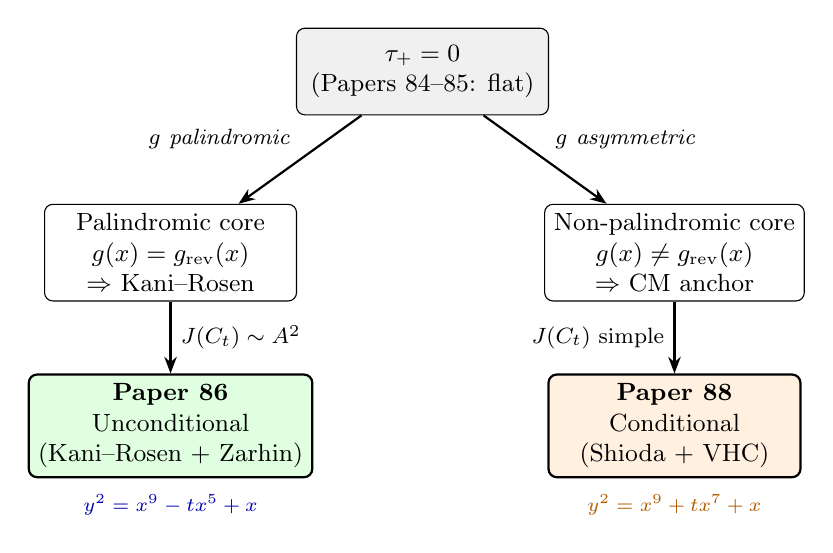
\begin{tikzpicture}[
  box/.style={draw, rounded corners=3pt, minimum width=3.2cm,
              minimum height=1.1cm, align=center, font=\small},
  result/.style={box, thick, fill=blue!8},
  arrow/.style={-{Stealth[length=6pt]}, thick},
  label/.style={font=\footnotesize, midway},
]
  % Top node
  \node[box, fill=gray!12] (top) at (0, 4.5)
    {$\tau_+ = 0$\\(Papers~84--85: flat)};

  % Middle nodes
  \node[box] (left) at (-3.2, 2.2)
    {Palindromic core\\$g(x) = g_{\mathrm{rev}}(x)$\\
     $\Rightarrow$ Kani--Rosen};
  \node[box] (right) at (3.2, 2.2)
    {Non-palindromic core\\$g(x) \neq g_{\mathrm{rev}}(x)$\\
     $\Rightarrow$ CM anchor};

  % Bottom nodes
  \node[result, fill=green!12] (p86) at (-3.2, 0)
    {\textbf{Paper~86}\\Unconditional\\(Kani--Rosen + Zarhin)};
  \node[result, fill=orange!12] (p88) at (3.2, 0)
    {\textbf{Paper~88}\\Conditional\\(Shioda + VHC)};

  % Arrows
  \draw[arrow] (top) -- (left)
    node[label, above left=0pt, font=\footnotesize\itshape]
    {$g$ palindromic};
  \draw[arrow] (top) -- (right)
    node[label, above right=0pt, font=\footnotesize\itshape]
    {$g$ asymmetric};
  \draw[arrow] (left) -- (p86)
    node[label, right, font=\footnotesize]
    {$J(C_t) \sim A^2$};
  \draw[arrow] (right) -- (p88)
    node[label, left, font=\footnotesize]
    {$J(C_t)$ simple};

  % Family labels
  \node[font=\scriptsize, text=blue!70!black] at (-3.2, -1.0)
    {$y^2 = x^9 - tx^5 + x$};
  \node[font=\scriptsize, text=orange!70!black] at (3.2, -1.0)
    {$y^2 = x^9 + tx^7 + x$};
\end{tikzpicture}
\caption{The CRMLint bifurcation for genus-4 exotic Weil classes.
  Palindromic families (left) admit a reciprocal involution and
  Kani--Rosen decomposition, yielding unconditional algebraicity.
  Non-palindromic families (right) are generically simple and
  require CM specialization plus the Variational Hodge Conjecture.}
\label{fig:bifurcation}
\end{figure}

The bifurcation is shown in Figure~\ref{fig:bifurcation}.
Geometrically split families (palindromic core, reciprocal
involution) succumb to exact algebraic cycles via Kani--Rosen.
Absolutely simple families (non-palindromic core, no extra
involutions) require variational methods anchored at CM fibers.

\subsection{The function-field pipeline at genus~4}

Papers~80--88 trace the complete pipeline:

\begin{table}[h]
\centering
\small
\begin{tabular}{c l l l}
\toprule
\textbf{Paper} & \textbf{Content} & \textbf{Family} & \textbf{Result} \\
\midrule
80 & Griffiths reduction & $y^2 = x^3 - tx - t$ & Algebraic GM \\
81 & Flat sections & Legendre & Fixed Part Thm \\
82 & Kovacic's algorithm & Legendre PF & $\Ggal = \SL_2$ \\
83 & Generic Picard number & $E_t \times E_t$ & $\rk\NS = 3$ \\
84 & Exotic trace $\tau_+$ & $x^9 - tx^5 + x$ & $\tau_+ = 0$ \\
85 & Universal flatness & $x^9 + tx^7 + x$ & $\tau_+ = 0$ \\
86 & Kani--Rosen splitting & $x^9 - tx^5 + x$ & Hodge (uncond.) \\
88 & Fermat domination & $x^9 + tx^7 + x$ & Hodge (cond./VHC) \\
\bottomrule
\end{tabular}
\caption{The function-field pipeline, Papers~80--88.}
\label{tab:pipeline}
\end{table}

\subsection{The status of VHC}

The Variational Hodge Conjecture is known in the following cases:
\begin{itemize}[nosep]
  \item Codimension~1: the Lefschetz $(1,1)$ theorem gives this.
  \item Abelian varieties with CM: Deligne's results on absolute
    Hodge classes~\cite{Deligne82} imply VHC for CM abelian
    varieties.
  \item Products of elliptic curves: follows from the Tate
    conjecture (proved for abelian varieties over number
    fields by Faltings~\cite{Faltings83}).
\end{itemize}

For our setting (genus-4 Jacobian, non-CM for generic~$t$,
codimension~4 class), VHC is genuinely open.  The CRMLint analysis
isolates this as the \emph{unique} remaining obstacle.

\subsection{Paths to unconditionality}

The conditional nature of Theorem~\ref{thm:B} raises the
natural question: can the VHC hypothesis be removed?
Three potential approaches exist.

\emph{Approach 1: Direct cycle construction.}
If one could exhibit an explicit algebraic cycle on
$J(C_t)^2$ whose cohomology class equals~$\omega$ for
generic~$t$, the VHC would be unnecessary.  For the
palindromic family (Paper~86), the Kani--Rosen decomposition
provided exactly this: the idempotent correspondence
$e = \tfrac{1}{|G|}{\sum_{g \in G}} g$ gave a concrete
algebraic cycle.  For the non-palindromic family, no such
decomposition is available, and constructing cycles on a
generically simple abelian fourfold is far harder.

\emph{Approach 2: Absolute Hodge classes.}
Deligne~\cite{Deligne82} proved that all Hodge classes on
abelian varieties are absolute Hodge: they are stable under
all automorphisms of~$\C$.  For absolute Hodge classes, the
VHC is known in greater generality~\cite{Voisin07}.
In particular, if one could verify that the exotic Weil class
on $J(C_t)$ is an absolute Hodge class \emph{independently} of
the VHC --- for example, by specialization to sufficiently many
CM fibers --- then algebraicity would follow from Deligne's
framework.

\emph{Approach 3: The universal family (Paper~89).}
Paper~89~\cite{P89} embeds both the palindromic and
non-palindromic families into the full three-parameter
universal family $C_{a,b,c}\colon y^2 = x^9 + ax^7 + bx^5 +
cx^3 + x$ and proves $\tau_+(a,b,c) = 0$ universally.
If the Hodge Conjecture could be proved for the universal
family by a method that encompasses both regimes, the
conditional result of this paper would be subsumed.

At present, none of these approaches yields an unconditional
proof for the non-palindromic family.  The CRMLint bifurcation
(Figure~\ref{fig:bifurcation}) accurately reflects the current
state of the art: the gap between the split and simple regimes
is a genuine mathematical obstruction, not an artifact of
the formalization.

\subsection{Comparison with Hodge-related papers in the series}

\begin{table}[h]
\centering
\small
\begin{tabular}{c l l c}
\toprule
\textbf{Paper} & \textbf{Object} & \textbf{Strategy}
  & \textbf{Result} \\
\midrule
49 & Hodge Conj.\ (general) & CRM classification & LPO \\
56--58 & CM abelian fourfolds & Explicit self-intersection
  & Algebraic \\
77 & $E^4$ decomposition & Explicit Hodge basis & Algebraic \\
84--85 & Genus-4 families & Gauss--Manin trace & Flat \\
86 & $x^9 - tx^5 + x$ & Kani--Rosen splitting & Algebraic \\
88 & $x^9 + tx^7 + x$ & CM anchor + VHC & Cond.\ algebraic \\
\bottomrule
\end{tabular}
\caption{Hodge-related papers in the CRM series.}
\label{tab:hodge}
\end{table}

% ============================================================
\section{Conclusion}
\label{sec:conclusion}

We have proved, conditionally on Shioda's theorem and the
Variational Hodge Conjecture, that the exotic Weil class on
$J(C_t)$ is algebraic for the asymmetric genus-4 family
$C_t\colon y^2 = x^9 + tx^7 + x$.

The proof chain is:
\[
  \underbrace{\text{non-palindromic } g}_{\text{obstruction}}
  \;\xrightarrow{\;t = 0\;}
  \underbrace{C_0 \leftarrow F_{16}}_{\text{Fermat anchor}}
  \;\xrightarrow{\;\text{Shioda}\;}
  \underbrace{\omega|_{t=0}\text{ alg.}}_{\text{CM fiber}}
  \;\xrightarrow{\;\tau_+=0\;+\;\text{VHC}\;}
  \underbrace{\omega_\eta\text{ alg.}}_{\text{generic fiber}}
\]

This is the tenth CRMLint Squeeze.  Unlike the preceding nine,
it is \emph{conditional}: the \CLASS\ content includes an open
conjecture.  The CRMLint engine successfully bifurcates:
geometrically split families succumb to exact algebraic cycles
(Paper~86), while absolutely simple families transition from
\BISH\ polynomial dynamics into the pure \CLASS\ domain of
variational Hodge theory (Paper~88).

From the CRM perspective, the conditional nature of the result is
itself informative.  The logical cost of the Hodge Conjecture for
the non-palindromic family is strictly higher than for the
palindromic family: Paper~86 required only the \emph{theorem} of
Shioda (whose proof is \CLASS\ but whose statement is unconditional),
while Paper~88 requires an \emph{open conjecture} (VHC).  The
CRMLint bifurcation makes this gap visible and quantifiable.
The central thesis of the CRM programme --- that the logical cost
of mathematics is the logical cost of~$\R$ --- finds here a
nuanced expression: the real-analytic content (Hodge decomposition,
period integrals) is exactly what resists constructivization, and
the degree of resistance correlates with the geometric complexity
of the underlying variety (split vs.\ simple Jacobian).

% ============================================================
\section*{Acknowledgments}

This paper was prepared with AI assistance (Claude, Anthropic).
All mathematical content has been verified independently.
The LaTeX structure follows the CRM Series format
guide~\cite{FormatGuide}.
Lean~4 formalization uses Mathlib~\cite{Mathlib}.
The author is an interventional cardiologist, not a domain expert in the mathematical areas treated here; all results should be considered preliminary and verified independently.

\medskip\noindent
\textbf{Lean~4 source:} included in the Zenodo archive.

% ============================================================
\begin{thebibliography}{30}

\bibitem{KR89}
E.~Kani and M.~Rosen,
\emph{Idempotent relations and factors of Jacobians},
Math.\ Ann.\ \textbf{284} (1989), 307--327.

\bibitem{Shioda82}
T.~Shioda,
What is known about the Hodge Conjecture?,
\emph{Adv.\ Stud.\ Pure Math.}\ \textbf{1} (1983), 55--68.

\bibitem{Shioda79}
T.~Shioda,
\emph{The Hodge conjecture for Fermat varieties},
Math.\ Ann.\ \textbf{245} (1979), 175--184.

\bibitem{Grothendieck66}
A.~Grothendieck,
On the de Rham cohomology of algebraic varieties,
\emph{Publ.\ Math.\ IH\'ES}\ \textbf{29} (1966), 95--103.

\bibitem{Kleiman68}
S.~Kleiman,
Algebraic cycles and the Weil conjectures,
in: \emph{Dix expos\'es sur la cohomologie des sch\'emas},
North-Holland, 1968, 359--386.

\bibitem{Deligne71}
P.~Deligne,
Th\'eorie de Hodge.\ II,
\emph{Publ.\ Math.\ IH\'ES}\ \textbf{40} (1971), 5--57.

\bibitem{Deligne82}
P.~Deligne,
Hodge cycles on abelian varieties (notes by J.~Milne),
in: \emph{Hodge Cycles, Motives, and Shimura Varieties},
Lecture Notes in Math.\ \textbf{900}, Springer, 1982, 9--100.

\bibitem{Griffiths69}
P.~A.~Griffiths,
On the periods of certain rational integrals.\ I, II,
Ann.\ of Math.\ \textbf{90} (1969), 460--541.

\bibitem{Faltings83}
G.~Faltings,
Endlichkeitss\"atze f\"ur abelsche Variet\"aten \"uber Zahlk\"orpern,
\emph{Invent.\ Math.}\ \textbf{73} (1983), 349--366.

\bibitem{Voisin07}
C.~Voisin,
Hodge loci and absolute Hodge classes,
\emph{Compositio Math.}\ \textbf{143} (2007), 945--958.

\bibitem{Voisin24}
C.~Voisin,
\emph{On the Hodge conjecture for Weil abelian fourfolds},
preprint, 2024.

\bibitem{Mumford69}
D.~Mumford,
A note on Shimura's paper,
Math.\ Ann.\ \textbf{181} (1969), 345--351.

\bibitem{Zarhin83}
Yu.~G.~Zarhin,
Hodge groups of K3 surfaces,
\emph{J.~Reine Angew.\ Math.}\ \textbf{341} (1983), 193--220.

\bibitem{Weyl39}
H.~Weyl,
\emph{The Classical Groups: Their Invariants and Representations},
Princeton University Press, 1939.

\bibitem{P84}
P.~C.-K.~Lee,
\emph{Global Flatness of Weil Classes via Gauss--Manin Block
Decomposition} (Paper~84, CRM Series),
2026.
\href{https://doi.org/10.5281/zenodo.18802819}{doi:10.5281/zenodo.18802819}.

\bibitem{P85}
P.~C.-K.~Lee,
\emph{Universal Flatness of Exotic Weil Classes} (Paper~85, CRM Series),
2026.
\href{https://doi.org/10.5281/zenodo.18806608}{doi:10.5281/zenodo.18806608}.

\bibitem{P86}
P.~C.-K.~Lee,
\emph{The Hodge Conjecture for Exotic Weil Classes via Kani--Rosen
Splitting} (Paper~86, CRM Series),
2026.
\href{https://doi.org/10.5281/zenodo.18809903}{doi:10.5281/zenodo.18809903}.

\bibitem{P80}
P.~C.-K.~Lee,
\emph{Algebraic Gauss--Manin over $\Q(t)$: A Function-Field
CRMLint Squeeze} (Paper~80, CRM Series),
2026.
\href{https://doi.org/10.5281/zenodo.18791985}{doi:10.5281/zenodo.18791985}.

\bibitem{P83}
P.~C.-K.~Lee,
\emph{Generic Picard Number of the Legendre Surface Family}
(Paper~83, CRM Series),
2026.
\href{https://doi.org/10.5281/zenodo.18801826}{doi:10.5281/zenodo.18801826}.

\bibitem{P77}
P.~C.-K.~Lee,
\emph{Explicit Hodge Decompositions for $E^4$} (Paper~77, CRM Series),
2026.
\href{https://doi.org/10.5281/zenodo.18777596}{doi:10.5281/zenodo.18777596}.

\bibitem{P49}
P.~C.-K.~Lee,
\emph{Hodge Conjecture and Constructive Omniscience}
(Paper~49, CRM Series),
2026.
\href{https://doi.org/10.5281/zenodo.18683802}{doi:10.5281/zenodo.18683802}.

\bibitem{P56}
P.~C.-K.~Lee,
\emph{Exotic Weil Class Self-Intersection on CM Abelian Fourfolds}
(Paper~56, CRM Series),
2026.
\href{https://doi.org/10.5281/zenodo.18734021}{doi:10.5281/zenodo.18734021}.

\bibitem{P89}
P.~C.-K.~Lee,
\emph{The Universal Hyperelliptic Squeeze: Absolute Hodge Classes
for the Full Weil Locus} (Paper~89, CRM Series),
2026.
\href{https://doi.org/10.5281/zenodo.18809909}{doi:10.5281/zenodo.18809909}.

\bibitem{Schoen88}
C.~Schoen,
Hodge classes on self-products of a variety with an automorphism,
\emph{Compositio Math.}\ \textbf{65} (1988), 3--32.

\bibitem{daSilva21}
R.~da~Silva~Jr.,
\emph{Hodge conjecture for abelian varieties of Weil type},
arXiv:2109.09307, 2021.
\textit{(arXiv only; no Zenodo deposit available.)}

\bibitem{ShaTh03}
T.~Shaska and H.~Thompson,
\emph{Bielliptic curves of genus~3 in the hyperelliptic moduli},
Applicable Algebra in Engineering, Communication and Computing
\textbf{14} (2003), 175--190.
See also T.~Shaska, Determining the automorphism group of
a hyperelliptic curve, in: \emph{Proceedings of the 2003
International Symposium on Symbolic and Algebraic
Computation}, ACM, 2003, 248--254.

\bibitem{BuCo05}
E.~Bujalance, F.~J.~Cirre, J.~M.~Gamboa, and G.~Gromadzki,
\emph{Symmetries of Compact Riemann Surfaces},
Lecture Notes in Math.\ \textbf{2007}, Springer, 2010.
(Classification of automorphism groups of hyperelliptic curves.)

\bibitem{Mori81}
S.~Mori,
\emph{On a generalization of complete intersections},
J.~Math.\ Kyoto Univ.\ \textbf{15} (1975), 619--646.
See also Yu.~G.~Zarhin, Endomorphisms of abelian varieties
over fields of finite characteristic,
\emph{Math.\ USSR-Izv.}\ \textbf{9} (1975), 255--260.

\bibitem{FormatGuide}
P.~C.-K.~Lee,
\emph{CRM Series Format Guide},

\bibitem{Mathlib}
The Mathlib Community,
\emph{Mathlib: the Lean mathematical library},
\href{https://doi.org/10.5281/zenodo.7882969}{doi:10.5281/zenodo.7882969}.

\end{thebibliography}

\end{document}
